\documentclass[11pt]{article}
\usepackage[margin=1in]{geometry}
\usepackage{amsmath,amssymb,amsthm}
\usepackage{bm}
\usepackage{graphicx}
\graphicspath{{figures/}{./}}
\usepackage{hyperref}
\usepackage{booktabs}
\usepackage{mathtools}
\usepackage{xcolor}

\hypersetup{colorlinks=true,linkcolor=blue,citecolor=blue,urlcolor=blue}

\newcommand{\E}{\mathbb{E}}
\newcommand{\R}{\mathbb{R}}
\newcommand{\N}{\mathcal{N}}
\newcommand{\KL}[2]{D_{\mathrm{KL}}\!\left(#1\,\|\,#2\right)}
\newcommand{\norm}[1]{\left\|#1\right\|}
\newcommand{\grad}{\nabla}
\newcommand{\abar}{\bar{\alpha}}
\newcommand{\tparam}{\theta}
\newcommand{\sth}{s_\theta}
\newcommand{\epsth}{\varepsilon_\theta}

\title{\textbf{EE/CS 148B HW4}\\\large Diffusion Models — Written Solutions}
\author{Alex Chung}
\date{Spring 2026}

\begin{document}
\maketitle

\tableofcontents
\newpage

%============================================================
\section{Part 1: DDPM — The Iterative Denoising Perspective}
%============================================================

\subsection{Problem 1.2: Variational Bound}

\textbf{Why minimize the variational bound on negative log likelihood.}

We wish to learn a generative model $p_\theta$ by maximizing the log-likelihood
$\E_{x_0 \sim q}[\log p_\theta(x_0)]$.  Because the latent-variable marginal
$p_\theta(x_0) = \int p_\theta(x_{0:T})\,dx_{1:T}$
involves an intractable integral over all latent trajectories, we derive a
tractable surrogate via Jensen's inequality.

\textbf{Proof of the chain of inequalities (Eq.~3 in DDPM).}

For any forward process $q(x_{1:T}\mid x_0)$, multiply and divide inside the
log to introduce $q$:
\begin{align*}
\log p_\theta(x_0)
&= \log \int p_\theta(x_{0:T})\,dx_{1:T}\\
&= \log \int \frac{p_\theta(x_{0:T})}{q(x_{1:T}\mid x_0)}\,
            q(x_{1:T}\mid x_0)\,dx_{1:T}\\
&= \log \E_{q(x_{1:T}\mid x_0)}\!\left[
      \frac{p_\theta(x_{0:T})}{q(x_{1:T}\mid x_0)}\right].
\end{align*}
Applying Jensen's inequality $\log\E[Z]\ge\E[\log Z]$ (since $\log$ is concave):
\begin{align*}
\log p_\theta(x_0)
&\ge \E_{q(x_{1:T}\mid x_0)}\!\left[
      \log\frac{p_\theta(x_{0:T})}{q(x_{1:T}\mid x_0)}\right].
\end{align*}
Negating and taking the expectation over $x_0\sim q(x_0)$ gives
\begin{align}
\E_q[-\log p_\theta(x_0)]
&\le \E_q\!\left[-\log\frac{p_\theta(x_{0:T})}{q(x_{1:T}\mid x_0)}\right]
 =: L. \label{eq:elbo}
\end{align}
Expanding the joint $p_\theta(x_{0:T})=p(x_T)\prod_{t=1}^{T}p_\theta(x_{t-1}\mid x_t)$
and the Markov chain $q(x_{1:T}\mid x_0)=\prod_{t=1}^{T}q(x_t\mid x_{t-1})$:
\begin{align*}
L &= \E_q\!\left[
      -\log p(x_T)
      - \sum_{t=1}^{T}\log\frac{p_\theta(x_{t-1}\mid x_t)}{q(x_t\mid x_{t-1})}
    \right],
\end{align*}
which equals Eq.~(3) of Ho et al.~(2020).

\textbf{Why we minimize $L$ rather than maximize $\log p_\theta(x_0)$:} $L$ is a
tractable upper bound on the NLL. Minimizing $L$ pushes the ELBO up, thereby
maximizing a guaranteed lower bound on $\log p_\theta(x_0)$.

\subsection{Problem 1.3: Tractable Loss Function}

We justify Equations (18), (20), (21), and (22) from Appendix~A of Ho et al.

\textbf{Eq.~(18): Closed-form posterior $q(x_{t-1}\mid x_t,x_0)$.}

By Bayes' rule and the Markov property:
\begin{equation}
q(x_{t-1}\mid x_t,x_0) \propto q(x_t\mid x_{t-1})\,q(x_{t-1}\mid x_0).
\end{equation}
Using
$q(x_t\mid x_{t-1}) = \N\!\bigl(x_t;\sqrt{\alpha_t}\,x_{t-1},\,\beta_t\mathbf{I}\bigr)$
and
$q(x_{t-1}\mid x_0) = \N\!\bigl(x_{t-1};\sqrt{\abar_{t-1}}\,x_0,\,(1-\abar_{t-1})\mathbf{I}\bigr)$,
taking the log of the product and completing the square in $x_{t-1}$:
\begin{align*}
\log q(x_{t-1}\mid x_t,x_0)
&\propto
  -\tfrac{1}{2}\!\left[
    \frac{(x_t - \sqrt{\alpha_t}\,x_{t-1})^2}{\beta_t}
    + \frac{(x_{t-1} - \sqrt{\abar_{t-1}}\,x_0)^2}{1-\abar_{t-1}}
  \right]\\
&= -\tfrac{1}{2}\!\left[
    \left(\frac{\alpha_t}{\beta_t}+\frac{1}{1-\abar_{t-1}}\right)x_{t-1}^2
    - 2\!\left(\frac{\sqrt{\alpha_t}}{\beta_t}x_t
              +\frac{\sqrt{\abar_{t-1}}}{1-\abar_{t-1}}x_0\right)x_{t-1}
    + C(x_t,x_0)
  \right].
\end{align*}
This is a Gaussian in $x_{t-1}$ with precision
$\sigma_{t}^{-2} = \frac{\alpha_t}{\beta_t}+\frac{1}{1-\abar_{t-1}}
= \frac{1-\abar_t}{\beta_t(1-\abar_{t-1})}$,
so
\begin{equation}
\tilde\beta_t := \sigma_{t}^2
= \frac{\beta_t(1-\abar_{t-1})}{1-\abar_t},
\qquad
\tilde\mu_t(x_t,x_0)
= \frac{\sqrt{\alpha_t}(1-\abar_{t-1})\,x_t + \sqrt{\abar_{t-1}}\,\beta_t\,x_0}{1-\abar_t}.
\tag{18}
\end{equation}
\textit{Theorem used}: Completion of the square for a Gaussian distribution; the product of two Gaussians is Gaussian (with precision equal to the sum of precisions).

\textbf{Eq.~(20): Reparameterised posterior mean.}

From Eq.~(6), $x_t = \sqrt{\abar_t}\,x_0 + \sqrt{1-\abar_t}\,\varepsilon$ gives
$x_0 = \bigl(x_t - \sqrt{1-\abar_t}\,\varepsilon\bigr)/\sqrt{\abar_t}$.
Substituting into Eq.~(18):
\begin{align*}
\tilde\mu_t
&= \frac{\sqrt{\alpha_t}(1-\abar_{t-1})x_t
  + \sqrt{\abar_{t-1}}\beta_t\,(x_t-\sqrt{1-\abar_t}\,\varepsilon)/\sqrt{\abar_t}}
         {1-\abar_t}.
\end{align*}
Using $\sqrt{\abar_{t-1}}/\sqrt{\abar_t} = 1/\sqrt{\alpha_t}$, the coefficient
of $x_t$ in the numerator is
$\sqrt{\alpha_t}(1-\abar_{t-1}) + \beta_t/\sqrt{\alpha_t}
= [\alpha_t(1-\abar_{t-1})+\beta_t]/\sqrt{\alpha_t}
= (1-\abar_t)/\sqrt{\alpha_t}$
(using $\alpha_t+\beta_t=1$ and $\abar_t=\alpha_t\abar_{t-1}$).
Therefore:
\begin{equation}
\tilde\mu_t(x_t,x_0)
= \frac{1}{\sqrt{\alpha_t}}\!\left(
    x_t - \frac{\beta_t}{\sqrt{1-\abar_t}}\,\varepsilon
  \right).
\tag{20}
\end{equation}
\textit{Equality used}: Eq.~(6), the reparameterisation $x_t = \sqrt{\abar_t}x_0 + \sqrt{1-\abar_t}\varepsilon$.

\textbf{Eq.~(21): $L_{t-1}$ as a mean squared error.}

Setting $\Sigma_\theta(x_t,t)=\sigma_t^2\mathbf{I}$ (fixed variance) and noting
that $q(x_{t-1}\mid x_t,x_0)=\N(\tilde\mu_t,\tilde\beta_t\mathbf{I})$ while
$p_\theta(x_{t-1}\mid x_t)=\N(\mu_\theta,\sigma_t^2\mathbf{I})$:
\begin{align}
L_{t-1}
&= \KL{q(x_{t-1}\mid x_t,x_0)}{p_\theta(x_{t-1}\mid x_t)} \notag\\
&= \frac{1}{2\sigma_t^2}\norm{\tilde\mu_t(x_t,x_0)-\mu_\theta(x_t,t)}^2
  +C', \tag{21}
\end{align}
dropping terms that do not depend on $\theta$.
\textit{Theorem used}: Closed-form KL divergence between two Gaussians with the same
(diagonal) covariance,
$\KL{\N(\mu_1,\Sigma)}{\N(\mu_2,\Sigma)}=\tfrac{1}{2}(\mu_1-\mu_2)^\top\Sigma^{-1}(\mu_1-\mu_2)$.

\textbf{Eq.~(22): Noise-parameterised simplified loss.}

Define $\mu_\theta(x_t,t) = \frac{1}{\sqrt{\alpha_t}}\bigl(x_t
- \frac{\beta_t}{\sqrt{1-\abar_t}}\,\epsth(x_t,t)\bigr)$.
Then
\begin{align*}
\norm{\tilde\mu_t - \mu_\theta}^2
&= \norm{
    \frac{1}{\sqrt{\alpha_t}}\!\left(x_t-\frac{\beta_t}{\sqrt{1-\abar_t}}\varepsilon\right)
   -\frac{1}{\sqrt{\alpha_t}}\!\left(x_t-\frac{\beta_t}{\sqrt{1-\abar_t}}\epsth\right)
   }^2\\
&= \frac{\beta_t^2}{\alpha_t(1-\abar_t)}\norm{\varepsilon-\epsth(x_t,t)}^2.
\end{align*}
Substituting into Eq.~(21) with $\sigma_t^2=\tilde\beta_t$ and taking the expectation:
\begin{equation}
L_{t-1} - C
= \E_{x_0,\varepsilon}\!\left[
    \frac{\beta_t^2}{2\sigma_t^2\alpha_t(1-\abar_t)}
    \norm{\varepsilon - \epsth\!\bigl(\sqrt{\abar_t}\,x_0+\sqrt{1-\abar_t}\,\varepsilon,\,t\bigr)}^2
  \right]. \tag{22}
\end{equation}

\subsection{Problem 1.4: Markov Process — Equation (4)}

\textbf{Claim:} The forward process is a Markov chain:
$q(x_{1:T}\mid x_0) = \prod_{t=1}^{T}q(x_t\mid x_{t-1})$.

\textbf{Proof:} By the chain rule of probability:
\begin{equation}
q(x_{1:T}\mid x_0)
= \prod_{t=1}^{T} q(x_t\mid x_{t-1},\ldots,x_0).
\end{equation}
The diffusion process is designed so that each step depends only on the previous
state: $q(x_t\mid x_{t-1},x_{t-2},\ldots,x_0) = q(x_t\mid x_{t-1})$.
This is the defining Markov property. Substituting:
\begin{equation}
q(x_{1:T}\mid x_0) = \prod_{t=1}^{T}q(x_t\mid x_{t-1}).
\end{equation}
Each transition is Gaussian:
$q(x_t\mid x_{t-1}) = \N\!\bigl(x_t;\sqrt{1-\beta_t}\,x_{t-1},\,\beta_t\mathbf{I}\bigr)$.

\subsection{Problem 1.5: Markov Process — Equations (6) and (7)}

\textbf{Eq.~(6): Marginal $q(x_t\mid x_0)$.}

We show by induction that $x_t = \sqrt{\abar_t}\,x_0 + \sqrt{1-\abar_t}\,\varepsilon$
with $\varepsilon\sim\N(0,\mathbf{I})$, where $\abar_t=\prod_{s=1}^{t}\alpha_s$ and $\alpha_s=1-\beta_s$.

\textit{Base case} ($t=1$): From the transition $x_1 = \sqrt{\alpha_1}x_0 + \sqrt{\beta_1}\varepsilon_1$, we have $\abar_1=\alpha_1$, which matches.

\textit{Inductive step}: Assume $x_{t-1} = \sqrt{\abar_{t-1}}x_0 + \sqrt{1-\abar_{t-1}}\varepsilon_{t-1}$.
Then:
\begin{align*}
x_t &= \sqrt{\alpha_t}\,x_{t-1} + \sqrt{\beta_t}\,\varepsilon_t\\
    &= \sqrt{\alpha_t\abar_{t-1}}\,x_0
       + \sqrt{\alpha_t(1-\abar_{t-1})}\,\varepsilon_{t-1}
       + \sqrt{\beta_t}\,\varepsilon_t.
\end{align*}
The two noise terms are independent Gaussians. By the additivity of Gaussian variances:
$\sqrt{\alpha_t(1-\abar_{t-1})}\,\varepsilon_{t-1} + \sqrt{\beta_t}\,\varepsilon_t
\stackrel{d}{=} \sqrt{\alpha_t(1-\abar_{t-1})+\beta_t}\,\varepsilon
= \sqrt{1-\abar_t}\,\varepsilon$,
where the last step uses $\abar_t = \alpha_t\abar_{t-1}$ and $\alpha_t+\beta_t=1$:
\[
\alpha_t(1-\abar_{t-1})+\beta_t
= \alpha_t - \alpha_t\abar_{t-1} + 1-\alpha_t
= 1-\abar_t.
\]
Therefore $q(x_t\mid x_0)=\N\!\bigl(x_t;\sqrt{\abar_t}\,x_0,\,(1-\abar_t)\mathbf{I}\bigr)$.

\textbf{Eq.~(7): Posterior $q(x_{t-1}\mid x_t,x_0)$.}

The posterior is derived via Bayes' rule using the joint distribution of
$(x_{t-1}, x_t)$ given $x_0$. Using the Gaussian conditioning formula:

Joint:
\[
\begin{pmatrix}x_{t-1}\\x_t\end{pmatrix}\bigg\vert\, x_0
\sim \N\!\left(
  \begin{pmatrix}\sqrt{\abar_{t-1}}x_0\\\sqrt{\abar_t}x_0\end{pmatrix},
  \begin{pmatrix}(1-\abar_{t-1})\mathbf{I} & \sqrt{\alpha_t}(1-\abar_{t-1})\mathbf{I}\\
                \sqrt{\alpha_t}(1-\abar_{t-1})\mathbf{I} & (1-\abar_t)\mathbf{I}\end{pmatrix}
\right).
\]
(The cross-covariance $\mathrm{Cov}(x_{t-1},x_t\mid x_0) = \sqrt{\alpha_t}(1-\abar_{t-1})\mathbf{I}$
follows from $x_t = \sqrt{\alpha_t}x_{t-1}+\sqrt{\beta_t}\varepsilon_t$
and $\mathrm{Var}(x_{t-1}\mid x_0)=(1-\abar_{t-1})\mathbf{I}$.)

By the Gaussian conditioning formula:
\begin{align*}
x_{t-1}\mid x_t, x_0 &\sim \N(\tilde\mu_t,\tilde\beta_t\mathbf{I}),\\
\tilde\mu_t &= \sqrt{\abar_{t-1}}x_0 + \sqrt{\alpha_t}(1-\abar_{t-1})\cdot
              \frac{x_t - \sqrt{\abar_t}x_0}{1-\abar_t}\\
            &= \frac{\sqrt{\alpha_t}(1-\abar_{t-1})x_t + \sqrt{\abar_{t-1}}\beta_t x_0}{1-\abar_t},\\
\tilde\beta_t &= (1-\abar_{t-1}) - \frac{\alpha_t(1-\abar_{t-1})^2}{1-\abar_t}
              = \frac{\beta_t(1-\abar_{t-1})}{1-\abar_t}.
\end{align*}

\subsection{Problem 1.6: KL Divergence and Equation (8)}

Setting $\Sigma_\theta(x_t,t)=\beta_t\mathbf{I}$ and using the closed-form KL formula
for two $k$-dimensional Gaussians $p=\N(\mu_p,\Sigma_p)$ and $q=\N(\mu_q,\Sigma_q)$
with $\Sigma_p=\Sigma_q=\beta_t\mathbf{I}$:
\begin{align*}
\KL{p}{q}
&= \frac{1}{2}\!\left[
    \log\frac{|\Sigma_q|}{|\Sigma_p|} - k
    + \mathrm{tr}(\Sigma_q^{-1}\Sigma_p)
    + (\mu_q-\mu_p)^\top\Sigma_q^{-1}(\mu_q-\mu_p)
  \right].
\end{align*}
When both distributions have the same covariance $\beta_t\mathbf{I}$, the first three terms
cancel (log ratio is 0, trace term is $k$, $-k$ cancels), leaving:
\begin{equation}
L_{t-1} = \KL{q(x_{t-1}\mid x_t,x_0)}{p_\theta(x_{t-1}\mid x_t)}
= \E_q\!\left[\frac{1}{2\beta_t}
              \norm{\tilde\mu_t(x_t,x_0)-\mu_\theta(x_t,t)}^2\right] + C. \tag{8}
\end{equation}
Here $C$ collects terms that do not depend on $\theta$ (e.g., constants from the log-determinant ratio and trace terms when the two covariances differ).

\subsection{Problem 1.7: Parameterization and Equation (12)}

Substituting the parameterization $\mu_\theta(x_t,t) = \frac{1}{\sqrt{\alpha_t}}\bigl(
x_t - \frac{\beta_t}{\sqrt{1-\abar_t}}\epsth(x_t,t)\bigr)$ into Eq.~(10)
(which is Eq.~(8) with $\sigma_t^2=\tilde\beta_t$):
\begin{align*}
\norm{\tilde\mu_t - \mu_\theta}^2
&= \left\|\frac{1}{\sqrt{\alpha_t}}\!\left(x_t - \frac{\beta_t}{\sqrt{1-\abar_t}}\varepsilon\right)
   -\frac{1}{\sqrt{\alpha_t}}\!\left(x_t - \frac{\beta_t}{\sqrt{1-\abar_t}}\epsth\right)\right\|^2\\
&= \frac{\beta_t^2}{\alpha_t(1-\abar_t)}\norm{\varepsilon - \epsth(x_t,t)}^2.
\end{align*}
Substituting into Eq.~(10) with $x_t = \sqrt{\abar_t}x_0 + \sqrt{1-\abar_t}\varepsilon$:
\begin{equation}
L_{t-1} - C
= \E_{x_0,\varepsilon}\!\left[
    \frac{\beta_t^2}{2\sigma_t^2\alpha_t(1-\abar_t)}
    \norm{\varepsilon - \epsth\!\bigl(\sqrt{\abar_t}\,x_0 + \sqrt{1-\abar_t}\,\varepsilon,\,t\bigr)}^2
  \right]. \tag{12}
\end{equation}

\subsection{Problem 1.8: Coefficient Plot}

The coefficient $\frac{\beta_t^2}{2\sigma_t^2\alpha_t(1-\abar_t)}$ (with $\sigma_t^2=\beta_t$)
is plotted in Figure~\ref{fig:coeff} using the linear schedule
$\beta_t\in[10^{-4},0.02]$, $T=1000$.

\begin{figure}[ht]
\centering
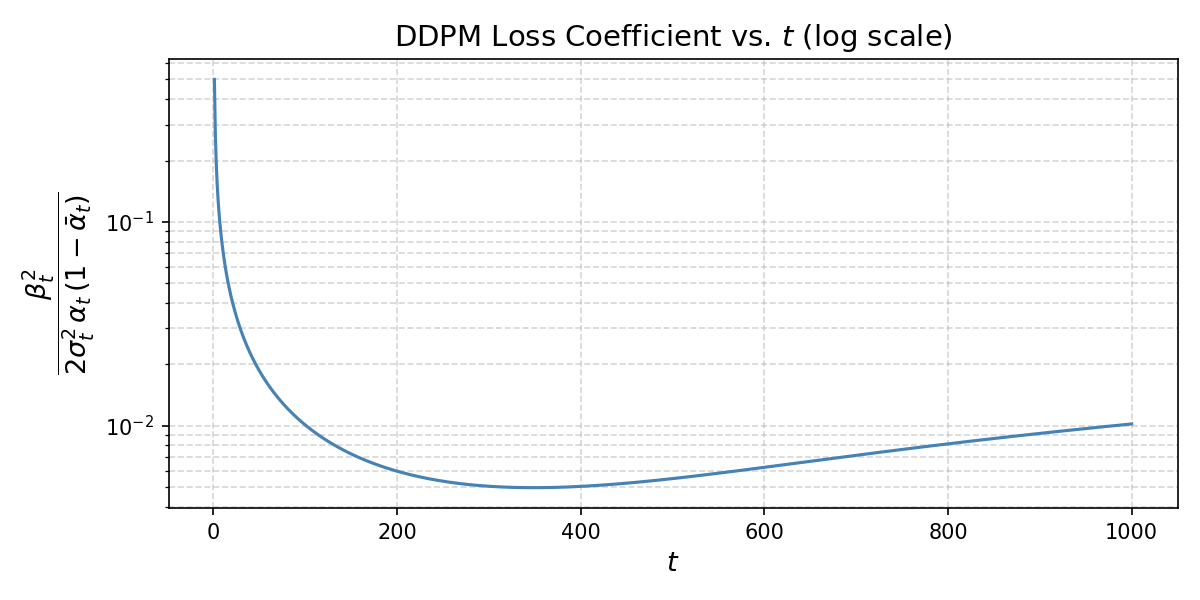
\includegraphics[width=0.78\textwidth]{coefficient_plot.png}
\caption{Loss coefficient $\beta_t^2/(2\sigma_t^2\alpha_t(1-\abar_t))$ vs.\ $t$
(log $y$-axis). The coefficient is much larger for small $t$ (low-noise,
fine detail) and very small for large $t$ (high-noise, coarse structure).
The simplified objective (which drops these weights) is thus equivalent to
down-weighting the fine-detail denoising terms.}
\label{fig:coeff}
\end{figure}

As noted in Section~3.4 of Ho et al., the simplified objective drops these
time-dependent weights, which empirically leads to better sample quality by
focusing training effort on the harder, high-noise timesteps.

%============================================================
\section{Part 2: Score Matching and Langevin Dynamics}
%============================================================

\subsection{Problem 2.2: Explicit Score Matching}

The explicit score matching (ESM) objective is:
\[
\mathcal{J}_\mathrm{ESM}(\theta)
= \E_{p(x)}\!\left[\tfrac{1}{2}\norm{\sth(x) - \nabla_x\log p(x)}^2\right].
\]
This is intractable in diffusion model applications for two reasons:
\begin{enumerate}
\item \textbf{Unknown data score}: The true score $\nabla_x\log p(x)$ of the data
distribution $p(x)$ is not available --- if it were, we would not need to learn it.
\item \textbf{Complex marginals}: In diffusion models, $p(x)$ at intermediate noise
levels is the marginal $p_t(x)=\int q(x\mid x_0)p_\mathrm{data}(x_0)\,dx_0$, whose
score is also unavailable in closed form for general data distributions.
\end{enumerate}

\subsection{Problem 2.3: Implicit Score Matching}

\textbf{Claim:} $\mathcal{J}_\mathrm{ESM}(\theta) = \mathcal{J}_\mathrm{ISM}(\theta) + C$
where $C$ does not depend on $\theta$ and
$\mathcal{J}_\mathrm{ISM}(\theta)
= \E_{p(x)}\!\bigl[\mathrm{tr}(\nabla_x\sth(x)) + \tfrac{1}{2}\norm{\sth(x)}^2\bigr]$.

\textbf{Proof:} Expanding the squared norm in ESM:
\begin{align*}
\mathcal{J}_\mathrm{ESM}(\theta)
&= \E_p\!\left[\tfrac{1}{2}\norm{\sth}^2
   - \sth(x)^\top\nabla_x\log p(x)
   + \tfrac{1}{2}\norm{\nabla_x\log p}^2\right].
\end{align*}
The last term is a constant $C$ independent of $\theta$. It remains to show
\[
\E_p\!\left[-\sth(x)^\top\nabla_x\log p(x)\right]
= \E_p\!\left[\mathrm{tr}(\nabla_x\sth(x))\right].
\]
Rewrite $\nabla_x\log p(x) = \frac{\nabla_x p(x)}{p(x)}$:
\begin{align*}
\E_p\!\left[-\sth(x)^\top\nabla_x\log p(x)\right]
&= -\int \sth(x)^\top\nabla_x p(x)\,dx.
\end{align*}
Apply vector integration by parts (Green's first identity), using $p(x)\to 0$ as $\|x\|\to\infty$:
\begin{align*}
-\int \sth(x)^\top\nabla_x p(x)\,dx
&= \int p(x)\,\mathrm{div}(\sth(x))\,dx
 = \E_p\!\left[\mathrm{tr}(\nabla_x\sth(x))\right].
\end{align*}
(The boundary term vanishes because $p$ vanishes at infinity.)
Therefore $\mathcal{J}_\mathrm{ESM} = \mathcal{J}_\mathrm{ISM} + C$. \qed

\subsection{Problem 2.4: Limitation of ISM}

Despite being tractable, ISM requires computing $\mathrm{tr}(\nabla_x\sth(x))$
--- the trace of the Jacobian of the network with respect to its input.  For a
network with $d$-dimensional input, this requires $d$ backward passes (one per
input dimension) or a Hutchinson estimator, making the per-step cost $O(d)$
times a standard gradient step.  For high-dimensional inputs such as images
($d=28\times28=784$ or larger), this is prohibitively expensive.  Furthermore,
estimating $\mathrm{tr}(\nabla_x\sth)$ via Hutchinson introduces additional
variance.

\subsection{Problem 2.5: Tweedie's Formula}

\textbf{Claim:} Given $\tilde x = x + \sigma\varepsilon$, $\varepsilon\sim\N(0,\mathbf{I})$,
$x\sim p(x)$:
\[
\E[x\mid\tilde x] = \tilde x + \sigma^2\,\nabla_{\tilde x}\log p_\sigma(\tilde x).
\]

\textbf{Proof:} Using the hint steps:

\textbf{Step 1:} We need $\E[x\mid\tilde x]$.  Since $\tilde x = \E[\tilde x\mid\tilde x]$:
\[
\E[x\mid\tilde x] = \tilde x - \E[\tilde x - x\mid\tilde x] = \tilde x - \E[\sigma\varepsilon\mid\tilde x].
\]

\textbf{Step 2:} Write the conditional expectation as an integral:
\[
\E[\sigma\varepsilon\mid\tilde x]
= \frac{\int \sigma\varepsilon\, p(\tilde x\mid x)\,p(x)\,dx}{p_\sigma(\tilde x)}
= \frac{\int (\tilde x - x)\, p(\tilde x\mid x)\,p(x)\,dx}{p_\sigma(\tilde x)}.
\]

\textbf{Step 3:} Note $p(\tilde x\mid x) = \N(\tilde x; x, \sigma^2\mathbf{I})$, so:
$\frac{\tilde x - x}{\sigma^2}\,p(\tilde x\mid x) = -\nabla_{\tilde x}p(\tilde x\mid x)$.
Applying Bayes' rule:
\[
\int (\tilde x-x)\,p(\tilde x\mid x)\,p(x)\,dx
= -\sigma^2 \int \nabla_{\tilde x}p(\tilde x\mid x)\,p(x)\,dx
= -\sigma^2\,\nabla_{\tilde x}p_\sigma(\tilde x).
\]

\textbf{Step 4:} Therefore:
\[
\E[\sigma\varepsilon\mid\tilde x] = \frac{-\sigma^2\,\nabla_{\tilde x}p_\sigma(\tilde x)}{p_\sigma(\tilde x)}
= -\sigma^2\,\nabla_{\tilde x}\log p_\sigma(\tilde x).
\]

\textbf{Conclusion:}
\[
\E[x\mid\tilde x] = \tilde x + \sigma^2\,\nabla_{\tilde x}\log p_\sigma(\tilde x). \qquad\square
\]

\subsection{Problem 2.6: DSM Objective from Tweedie's Formula}

\textbf{Training objective from Tweedie:} Tweedie tells us $\E[x\mid\tilde x] = \tilde x + \sigma^2\nabla_{\tilde x}\log p_\sigma(\tilde x)$.  We can therefore train $\sth(\tilde x)$ to approximate the score by regressing onto the known quantity $(\E[x\mid\tilde x]-\tilde x)/\sigma^2 = \nabla_{\tilde x}\log p_\sigma(\tilde x)$.  Since the conditional expectation is not directly accessible, we instead minimize:
\[
\mathcal{J}_\mathrm{train}(\theta;\sigma)
= \E_{p(x)}\E_{p(\tilde x\mid x)}\!\left[\tfrac{1}{2}\norm{\sth(\tilde x) - \nabla_{\tilde x}\log p(\tilde x\mid x)}^2\right],
\]
which is the DSM objective
$\mathcal{J}_\mathrm{DSM}(\theta;\sigma)
= \E_{p(x)}\E_{p(\tilde x\mid x)}\!\bigl[\tfrac{1}{2}\norm{\sth(\tilde x)-\nabla_{\tilde x}\log p(\tilde x\mid x)}^2\bigr]$.

\textbf{Proof of equivalence with ESM:}
Expand:
\begin{align*}
\mathcal{J}_\mathrm{DSM}
&= \E\!\left[\tfrac{1}{2}\norm{\sth(\tilde x)}^2
            - \sth(\tilde x)^\top\nabla_{\tilde x}\log p(\tilde x\mid x)
            + \tfrac{1}{2}\norm{\nabla_{\tilde x}\log p(\tilde x\mid x)}^2\right].
\end{align*}
The last term is $C$ independent of $\theta$. For the cross term, noting
$\nabla_{\tilde x}\log p(\tilde x\mid x)=-(\tilde x - x)/\sigma^2$:
\begin{align*}
\E_{\tilde x,x}\!\left[-\sth(\tilde x)^\top\nabla_{\tilde x}\log p(\tilde x\mid x)\right]
&= \E_{\tilde x}\!\left[\sth(\tilde x)^\top
    \underbrace{\E_x\!\left[\frac{\tilde x-x}{\sigma^2}\bigg|\tilde x\right]}_{%
    = -\nabla_{\tilde x}\log p_\sigma(\tilde x)\ \text{(from score identity)}}\right]\\
&= -\E_{\tilde x}\!\left[\sth(\tilde x)^\top\nabla_{\tilde x}\log p_\sigma(\tilde x)\right]\\
&= \E_{\tilde x}\!\left[\mathrm{tr}(\nabla_{\tilde x}\sth(\tilde x))\right]
   \quad\text{(by integration by parts, as in ISM)}.
\end{align*}
Thus $\mathcal{J}_\mathrm{DSM} = \mathcal{J}_\mathrm{ISM} + C = \mathcal{J}_\mathrm{ESM} + C$. \qed

\subsection{Problem 2.7: DSM vs.\ DDPM}

Setting $x=\alpha_t x_0$, $\tilde x = x_t$, $\sigma=\sqrt{1-\abar_t}$, the
DSM objective at noise level $\sigma=\sqrt{1-\abar_t}$ becomes:
\[
\mathcal{J}_\mathrm{DSM}
= \E\!\left[\tfrac{1}{2}\norm{\sth(x_t) - \nabla_{x_t}\log q(x_t\mid x_0)}^2\right].
\]
Since $\nabla_{x_t}\log q(x_t\mid x_0) = -\varepsilon/\sqrt{1-\abar_t}$, we have
$\sth^*(x_t) = -\varepsilon^*/\sqrt{1-\abar_t}$.
The simplified DDPM objective at time $t$ is:
$\norm{\varepsilon-\epsth(x_t,t)}^2$,
whose minimizer satisfies $\epsth^*(x_t,t)=\varepsilon^*$.
Therefore:
\[
s_{\theta^*}(x_t) = -\frac{\epsth^*(x_t,t)}{\sqrt{1-\abar_t}},
\quad\text{i.e.,}\quad
s_{\theta^*} = c(\sigma)\,\epsth^*, \quad c(\sigma) = -\frac{1}{\sigma} = -\frac{1}{\sqrt{1-\abar_t}}.
\]
The two objectives share the same optimizer, differing by the constant scalar $c(\sigma)=-1/\sigma$.

\subsection{Problem 2.8: Langevin Dynamics Sampling}

The overdamped Langevin SDE $dx_t = \nabla\log p_\sigma(x_t)\,dt + \sqrt{2}\,dB_t$
admits $p_\sigma(x)$ as its stationary distribution. For small $\sigma$, $p_\sigma\approx p$.

\textbf{Algorithm:}
\begin{enumerate}
\setlength{\itemsep}{0pt}
\item Train a score model $\sth(\tilde x)\approx\nabla_{\tilde x}\log p_\sigma(\tilde x)$
      via DSM with a small noise level $\sigma$.
\item Initialize $x_0\sim\N(0,\mathbf{I})$ (or any distribution).
\item For $k=0,1,\ldots,K-1$ (with step size $\eta>0$):
      \[x_{k+1} = x_k + \eta\,\sth(x_k) + \sqrt{2\eta}\,z_k,\quad z_k\sim\N(0,\mathbf{I}).\]
\item Return $x_K$ as an approximate sample from $p(x)$.
\end{enumerate}
As $K\to\infty$ (and $\eta\to0$ appropriately), $x_K\sim p_\sigma\approx p$.

%============================================================
\section{Part 3: The SDE Perspective of Diffusion Models}
%============================================================

\subsection{Problem 3.2: VP-SDE Approximations}

In Appendix~B of Song et al.\ (2021), the DDPM forward process with $x_{i+1}=\sqrt{1-\beta_i}x_i+\sqrt{\beta_i}z_i$ is shown to approximate the VP-SDE
$dx = -\tfrac{1}{2}\beta(t)x\,dt + \sqrt{\beta(t)}\,dB_t$
via two approximations as $\Delta t\ll 1$:

\begin{enumerate}
\item $\sqrt{1-\beta_i} \approx 1 - \tfrac{1}{2}\beta_i$. \quad
      This holds since $\sqrt{1-\beta}\approx 1-\beta/2$ for $\beta\ll 1$ (first-order Taylor expansion of $\sqrt{1-\beta}$ around $\beta=0$).  The error is $O(\beta^2)=O(\Delta t^2)$, which vanishes as $\Delta t\to 0$.

\item $\sqrt{\beta_i} \approx \sqrt{\beta(t)\Delta t}$. \quad
      With $\beta_i = \bar\beta_i\Delta t$ (the discrete noise level set proportional to $\Delta t$ so that the continuous limit is finite), and $\bar\beta_i\to\beta(t)$ as $\Delta t\to 0$, we get $\sqrt{\beta_i}=\sqrt{\bar\beta_i\Delta t}\approx\sqrt{\beta(t)\Delta t}$.  This is the standard It\^o SDE discretization term $g\sqrt{\Delta t}$.
\end{enumerate}

Under these two approximations the discrete update $x_{i+1}=\sqrt{1-\beta_i}x_i+\sqrt{\beta_i}z_i$ becomes $x_{t+\Delta t} = x_t - \tfrac{1}{2}\beta(t)x_t\,\Delta t + \sqrt{\beta(t)\Delta t}\,z$, which is exactly the Euler-Maruyama discretization of the VP-SDE.

\subsection{Problem 3.3: Reverse VP-SDE}

The general formula for the reverse SDE of $dx=f(x,t)\,dt+g(t)\,dB_t$ is
(Anderson, 1982; Song et al.\ Eq.~(6)):
\[
dx = \bigl[f(x,t) - g(t)^2\,\nabla_x\log p_t(x)\bigr]\,dt + g(t)\,d\bar B_t,
\]
where $d\bar B_t$ is the time-reversed Brownian motion.  For the VP-SDE with
$f(x,t)=-\tfrac{1}{2}\beta(t)x$ and $g(t)=\sqrt{\beta(t)}$:
\begin{equation}\boxed{
dx = \left[-\tfrac{1}{2}\beta(t)\,x
           - \beta(t)\,\nabla_x\log p_t(x)\right]dt
     + \sqrt{\beta(t)}\,d\bar B_t.}
\label{eq:revvp}
\end{equation}

\subsection{Problem 3.4: Reverse VP-SDE Discretization}

\textbf{Step 1: Discretize Eq.~(\ref{eq:revvp}).}

With $\beta_i=\bar\beta_i\Delta t$ and indices running from high noise ($i+1$) to low noise ($i$):
\begin{align}
x_i &= x_{i+1} - \Delta t\!\left[-\tfrac{1}{2}\beta(t_{i+1})x_{i+1}
                                   -\beta(t_{i+1})s_\theta(x_{i+1},i+1)\right]
        + \sqrt{\beta(t_{i+1})\Delta t}\,z_{i+1} \notag\\
    &= x_{i+1} + \tfrac{1}{2}\beta_{i+1}x_{i+1}
       + \beta_{i+1}s_\theta(x_{i+1},i+1)
       + \sqrt{\beta_{i+1}}\,z_{i+1}. \label{eq:disc1}
\end{align}

\textbf{Step 2: Substitute $s_\theta$.} Keep $s_\theta(x_{i+1},i+1)$.

\textbf{Step 3: Rearrange.} From Eq.~(\ref{eq:disc1}):
\[
x_i = (1+\tfrac{1}{2}\beta_{i+1})\,x_{i+1} + \beta_{i+1}s_\theta + \sqrt{\beta_{i+1}}z_{i+1}.
\]

\textbf{Step 4: Follow Appendix~E of Song21.} For $\beta_{i+1}\to 0$:
$1+\tfrac{1}{2}\beta_{i+1}\approx\frac{1}{\sqrt{1-\beta_{i+1}}}$ (Taylor expansion).
Rearranging the $x_{i+1}+\beta_{i+1}s_\theta$ part:
\begin{equation}\boxed{
x_i = \frac{1}{\sqrt{1-\beta_{i+1}}}\bigl(x_{i+1}+\beta_{i+1}s_\theta(x_{i+1},i+1)\bigr)
      + \sqrt{\beta_{i+1}}\,z_{i+1}.}
\end{equation}

\subsection{Problem 3.5: Connecting SDE and DDPM}

DDPM Algorithm~2 uses the update (with $\alpha_t=1-\beta_t$, $\sigma_t=\sqrt\beta_t$):
\[
x_{t-1} = \frac{1}{\sqrt{\alpha_t}}\!\left(x_t
  - \frac{\beta_t}{\sqrt{1-\abar_t}}\,\epsth(x_t,t)\right) + \sigma_t z.
\]
The VP-SDE update above has coefficient $\beta_{i+1}$ in front of $s_\theta$,
whereas DDPM has $\beta_t/\sqrt{1-\abar_t}$ in front of $\epsth$, divided by
$\sqrt{\alpha_{t}}$.  These are consistent because (from Problem~2.7):
\[
s_\theta(x_t,t) = -\frac{\epsth(x_t,t)}{\sigma(t)},
\]
where $\sigma(t)=\sqrt{1-\abar_t}$ is the standard deviation of the noise added
to $x_0$.  Substituting and noting $\beta_{i+1}/(1-\abar_t)^{1/2} \cdot (1-\abar_t)^{1/2}$ matches the DDPM factor, the two update rules agree up to the scalar $c(\sigma)=-1/\sigma$ from Problem~2.7.

\subsection{Problem 3.6: Reverse SDE vs.\ Langevin Dynamics}

\textbf{Extra information in the reverse SDE.}
Langevin dynamics uses only the marginal score $\nabla_x\log p(x)$ to sample from $p(x)$.
The reverse VP-SDE uses the \emph{time-indexed} score $\nabla_x\log p_t(x)$, which encodes
how the data distribution evolves under a structured noise process.  Specifically, it knows
that the process starts as $\N(0,\sigma_T^2\mathbf{I})$ at $t=T$ and approaches $p_\mathrm{data}$
as $t\to 0$, giving a principled annealing schedule.

\textbf{Reflection in the score matching objective (Song21 Eq.~7).}
The VP-SDE training objective is
$\E_t[\lambda(t)\E_{x_0,x_t}[\|s_\theta(x_t,t)+\varepsilon/\sigma(t)\|^2]]$,
which trains $s_\theta$ at \emph{every noise level $t$} to match the time-conditioned
score.  Langevin dynamics would only train at a single (small) $\sigma$.

\textbf{Reflection in the DDPM training objective (Ho et al.\ Eq.~14).}
DDPM trains $\epsth(x_t,t)$ at every discrete time step $t\in\{1,\ldots,T\}$,
explicitly conditioning on $t$.  The time index carries the information about
the current noise level, enabling the model to guide the reverse trajectory
accurately rather than blindly following the gradient of a single stationary distribution.

\subsection{Problem 3.7: Conditional Diffusion and Classifier Guidance}

The reverse SDE for the conditional distribution $p(x\mid y)$ is:
\[
dx = \bigl[f(x,t) - g(t)^2\,\nabla_x\log p_t(x\mid y)\bigr]\,dt + g(t)\,d\bar B_t.
\]
By Bayes' rule:
$\nabla_x\log p_t(x\mid y) = \nabla_x\log p_t(x) + \nabla_x\log p_t(y\mid x)$.

\textbf{Classifier guidance intuition.}
Train the unconditional score model $s_\theta(x,t)\approx\nabla_x\log p_t(x)$
and a \emph{noisy classifier} $p_\phi(y\mid x_t,t)$ separately.
At sampling time, combine:
$\nabla_x\log p_t(x\mid y) \approx s_\theta(x_t,t) + \nabla_{x_t}\log p_\phi(y\mid x_t,t)$.
The classifier gradient steers the sample toward the desired class $y$ while the
unconditional score ensures image quality.  Increasing the classifier gradient
weight (guidance scale) trades diversity for class fidelity.

%============================================================
\section{Part 4: Rectified Flow — Theory}
%============================================================

\subsection{Problem 4.1: Optimal Velocity Field}

\textbf{Claim:} The minimizer of
$\mathcal{L}_\mathrm{RF}(\theta) = \int_0^1\E\bigl[\|(X_1-X_0)-v_\theta(X_t,t)\|^2\bigr]\,dt$
is $v^*(x,t) = \E[X_1-X_0\mid X_t=x]$.

\textbf{Proof:} For fixed $t$, expand $\E[\|(X_1-X_0)-v_\theta(X_t,t)\|^2]$ by conditioning on $X_t$:
\begin{align*}
\E\bigl[\|(X_1-X_0)-v_\theta(X_t,t)\|^2\bigr]
&= \E_{X_t}\!\left[\E\bigl[\|(X_1-X_0)-v_\theta(X_t,t)\|^2\;\big|\;X_t\bigr]\right].
\end{align*}
For each fixed $X_t=x$, minimize over $v_\theta(x,t)$:
\begin{align*}
\frac{\partial}{\partial v}\,
\E\bigl[\|(X_1-X_0)-v\|^2\mid X_t=x\bigr]
&= 2\bigl(v - \E[X_1-X_0\mid X_t=x]\bigr) = 0\\
\Longrightarrow\quad v^*(x,t) &= \E[X_1-X_0\mid X_t=x]. \qquad\square
\end{align*}
(This is the pointwise conditional mean: for each $x$ and $t$, the velocity that
minimizes the squared error is the conditional expectation of the target.)

\subsection{Problem 4.2: Connection to Score Matching}

\textbf{Claim:} If $X_0\sim\N(0,\mathbf{I})$ and $p_t$ is the marginal density of $X_t=(1-t)X_0+tX_1$, then
\[
v^*(x,t) = \frac{x - \E[X_0\mid X_t=x]}{t}.
\]

\textbf{Derivation:} From the interpolation $X_t=(1-t)X_0+tX_1$:
$X_1 = (X_t-(1-t)X_0)/t$, so
\begin{align*}
v^*(x,t) &= \E[X_1-X_0\mid X_t=x]
           = \E\!\left[\frac{X_t-(1-t)X_0}{t}-X_0\,\bigg|\,X_t=x\right]\\
          &= \frac{x}{t} - \frac{1-t}{t}\E[X_0\mid X_t=x] - \E[X_0\mid X_t=x]
           = \frac{x - \E[X_0\mid X_t=x]}{t}.
\end{align*}

\textbf{Relating $\E[X_0\mid X_t=x]$ to the score via Tweedie's formula:}

Since $X_0\sim\N(0,\mathbf{I})$ and $X_t=tX_1+(1-t)X_0$, conditioning on $X_1=x_1$:
$X_t\mid X_1=x_1\sim\N(tx_1,(1-t)^2\mathbf{I})$.
The marginal score satisfies:
\begin{align*}
\nabla_x\log p_t(x)
&= \E_{X_1\mid X_t=x}\!\left[\nabla_x\log p(x\mid X_1)\right]
 = \E_{X_1\mid X_t=x}\!\left[-\frac{x-tX_1}{(1-t)^2}\right]\\
&= -\frac{x-t\,\E[X_1\mid X_t=x]}{(1-t)^2}.
\end{align*}
Using the constraint $t\E[X_1\mid X_t=x] = x-(1-t)\E[X_0\mid X_t=x]$
(from $\E[X_t\mid X_t=x]=x$):
\[
\nabla_x\log p_t(x)
= -\frac{(1-t)\E[X_0\mid X_t=x]}{(1-t)^2}
= -\frac{\E[X_0\mid X_t=x]}{1-t}.
\]
Therefore:
\[
\E[X_0\mid X_t=x] = -(1-t)\,\nabla_x\log p_t(x),
\]
and the optimal velocity is:
\begin{equation}\boxed{
v^*(x,t) = \frac{x + (1-t)\,\nabla_x\log p_t(x)}{t}.}
\end{equation}

\textbf{Discussion:} This reveals a direct connection between rectified flow and
score-based diffusion: the optimal rectified flow velocity at time $t$ is a linear
combination of $x$ and the score $\nabla\log p_t(x)$.  In particular, learning the
velocity field $v_\theta$ is equivalent to learning the score (up to a time-dependent
linear transform), so rectified flow and DDPM/VP-SDE are learning essentially the same
function.

\subsection{Problem 4.3: Straightness and Reflow}

\textbf{(1) Geometric meaning of $S$.}

The straightness metric $S = 1 - \frac{\E[\int_0^1\|v_\theta(X_t,t)\,dt-(X_1-X_0)\|^2\,dt]}{\E[\|X_1-X_0\|^2]}$
(where the numerator integral is $\E[\|\int_0^1 v_\theta dt - (X_1-X_0)\|^2]$).

\begin{itemize}
\item $S=1$: The numerator is zero, meaning $\int_0^1 v_\theta(X_t,t)\,dt = X_1-X_0$ exactly for all samples.  The ODE trajectory from $X_0$ to $X_1$ is a \emph{straight line}, so one Euler step suffices.
\item $S=0$: The integral of the velocity equals zero contribution on average relative to the true displacement; the trajectory is maximally curved, requiring many steps.
\end{itemize}

\textbf{(2) Why reflow produces straighter trajectories.}

After training the initial $v_\theta$, the ODE flow $\Phi^1(X_0)$ maps fresh noise to approximate data. The reflow procedure generates new pairs $(\hat X_0, \hat X_1)$ where $\hat X_0$ and $\hat X_1=\Phi^1(\hat X_0)$ are \emph{deterministically} coupled through the ODE.  The optimal velocity for these paired samples is $\hat X_1-\hat X_0$ pointwise (since the pairing is deterministic, the conditional expectation collapses).  Retraining on these pairs thus learns a velocity that better aligns with the straight-line path from $\hat X_0$ to $\hat X_1$, reducing the curvature of the ODE.  In other words, the initial $v_\theta$ already has implicit pairing between noise and data; reflow makes this pairing \emph{explicit} so that the new velocity can match it with fewer steps.

\textbf{(3) Computational cost of reflow.}

Each round of reflow requires: (a)~generating $N$ pairs by running $K$-step Euler ODE at inference ($O(NK)$ model evaluations), and (b)~retraining for several epochs.  In total, this is $\approx 2\times$ the original training cost per round.  The main reason to limit rounds is diminishing returns: each reflow round reduces the sampling steps needed roughly from $K$ to $K/r$ for some $r<2$, but the cost grows linearly.  Also, the generated $(\hat X_0,\hat X_1)$ pairs are approximate, and repeated reflow may compound approximation errors.

\subsection{Problem 4.4: Rectified Flow vs.\ DDPM}

\textbf{(1) Training objective.}
DDPM regresses the added noise $\varepsilon\in\N(0,\mathbf{I})$: $\|\varepsilon-\epsth(\sqrt{\abar_t}x_0+\sqrt{1-\abar_t}\varepsilon,\,t)\|^2$.
Rectified flow regresses the velocity $X_1-X_0$: $\|(X_1-X_0)-v_\theta(X_t,t)\|^2$.
DDPM's target is pure Gaussian noise, while rectified flow's target is a data-dependent vector.

\textbf{(2) Inference cost.}
DDPM requires $T\approx1000$ reverse steps because each step only removes a small $\beta_t$ fraction of noise and the SDE trajectory is stochastic and curved.  Rectified flow can use far fewer steps because the ODE trajectory is (approximately) straight; after reflow it can use exactly one Euler step, since the learned velocity field is constant along straight-line paths.

\textbf{(3) Trajectory geometry.}
DDPM's reverse process follows a stochastic curved SDE path, leading to large discretization error for large step sizes.  Rectified flow integrates a deterministic ODE along approximately straight trajectories, so the Euler method has small discretization error even with one or a few steps.

\textbf{(4) Likelihood evaluation.}
DDPM's ELBO gives a variational lower bound on $\log p(x)$, enabling tractable likelihood estimation.  Rectified flow, as a continuous normalizing flow via the ODE, can in principle compute exact log-likelihoods using the change-of-variables formula (instantaneous change of variables), but in practice this is expensive (requires trace of the Jacobian).  The standard rectified flow training does not provide a direct likelihood estimate.

%============================================================
\section{Part 5: VP-SDE Written Questions}
%============================================================

\subsection{Problem 4.A.i: Drift and Diffusion Coefficients}

For the VP-SDE $dx = f(x,t)\,dt + g(t)\,dB_t$:
\begin{align}
f(x,t) &= -\tfrac{1}{2}\beta(t)\,x, \\
g(t)   &= \sqrt{\beta(t)},
\end{align}
where $\beta(t)=\beta_\mathrm{min}+(\beta_\mathrm{max}-\beta_\mathrm{min})\,t$ is the
linear noise schedule (Eq.~(32) of Song21).

\subsection{Problem 5.A.ii: $\beta(t)$ and $c(t)$}

\textbf{$\beta(t)$:} Linear schedule (Song21 Eq.~32):
\[
\beta(t) = \beta_\mathrm{min} + (\beta_\mathrm{max}-\beta_\mathrm{min})\,t.
\]

\textbf{$c(t)$:} The signal decay factor (Song21 Eq.~33):
\[
c(t) = \exp\!\left(-\tfrac{1}{2}\int_0^t\beta(s)\,ds\right)
= \exp\!\left(-\tfrac{1}{2}\!\left[\beta_\mathrm{min}\,t
  + \tfrac{1}{2}(\beta_\mathrm{max}-\beta_\mathrm{min})\,t^2\right]\right).
\]
Consequently $\sigma(t)=\sqrt{1-c(t)^2}$, and the marginal is
$x_t = c(t)x_0 + \sigma(t)\varepsilon$, $\varepsilon\sim\N(0,\mathbf{I})$.

%============================================================
\section{Part 5: VP-SDE Experimental Results}
%============================================================

\subsection{Problem 5.C.i: Dataset Visualization}

FashionMNIST contains $70{,}000$ grayscale images ($28\times 28$ pixels, 1 channel)
across 10 clothing classes: T-shirt/top, Trouser, Pullover, Dress, Coat, Sandal,
Shirt, Sneaker, Bag, Ankle boot.  Sample images are shown in Figure~\ref{fig:fashion}.

\begin{figure}[ht]
\centering
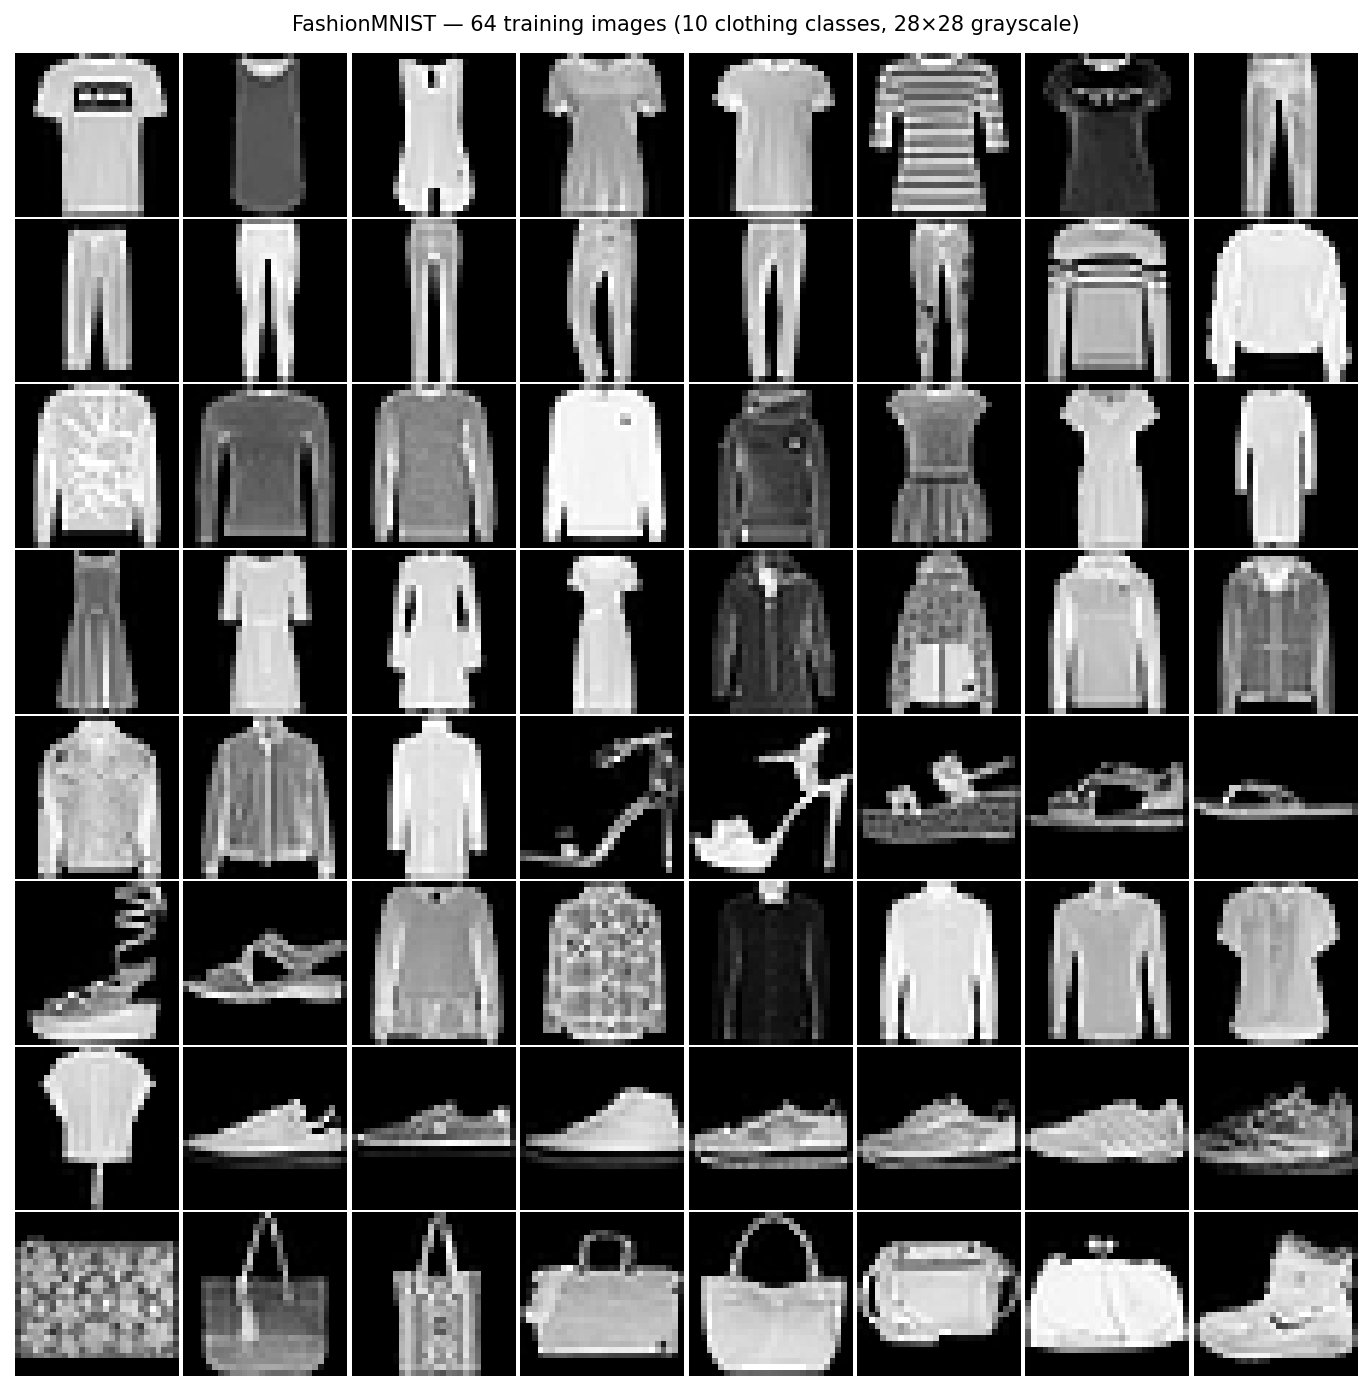
\includegraphics[width=0.85\textwidth]{fashion_grid.png}
\caption{64 FashionMNIST training images arranged in an 8$\times$8 grid.
Each image is $28\times28$ grayscale. The dataset spans 10 clothing classes:
T-shirt/top, Trouser, Pullover, Dress, Coat, Sandal, Shirt, Sneaker, Bag, Ankle boot.}
\label{fig:fashion}
\end{figure}

\subsection{Problem 5.C.ii: Training Curves}

\begin{figure}[ht]
\centering
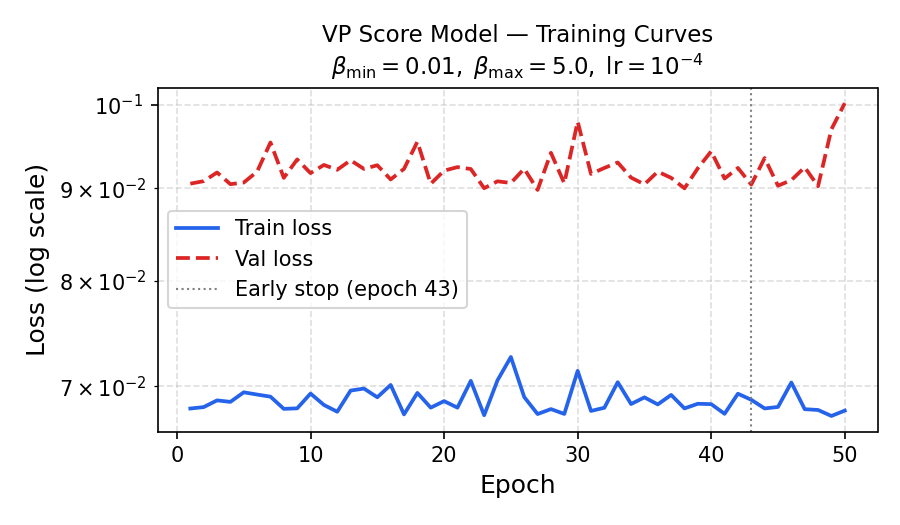
\includegraphics[width=0.78\textwidth]{vp_training_curves.png}
\caption{VP score model training and validation loss (log scale) over 50 epochs.
$\beta_\mathrm{min}=0.01$, $\beta_\mathrm{max}=5.0$, lr$=10^{-4}$, batch size$=128$.
Early stopping with patience$=10$ was applied (stopped at epoch 43).}
\label{fig:vp_loss}
\end{figure}

\subsection{Problem 5.C.iii: EM Samples}

\begin{figure}[ht]
\centering
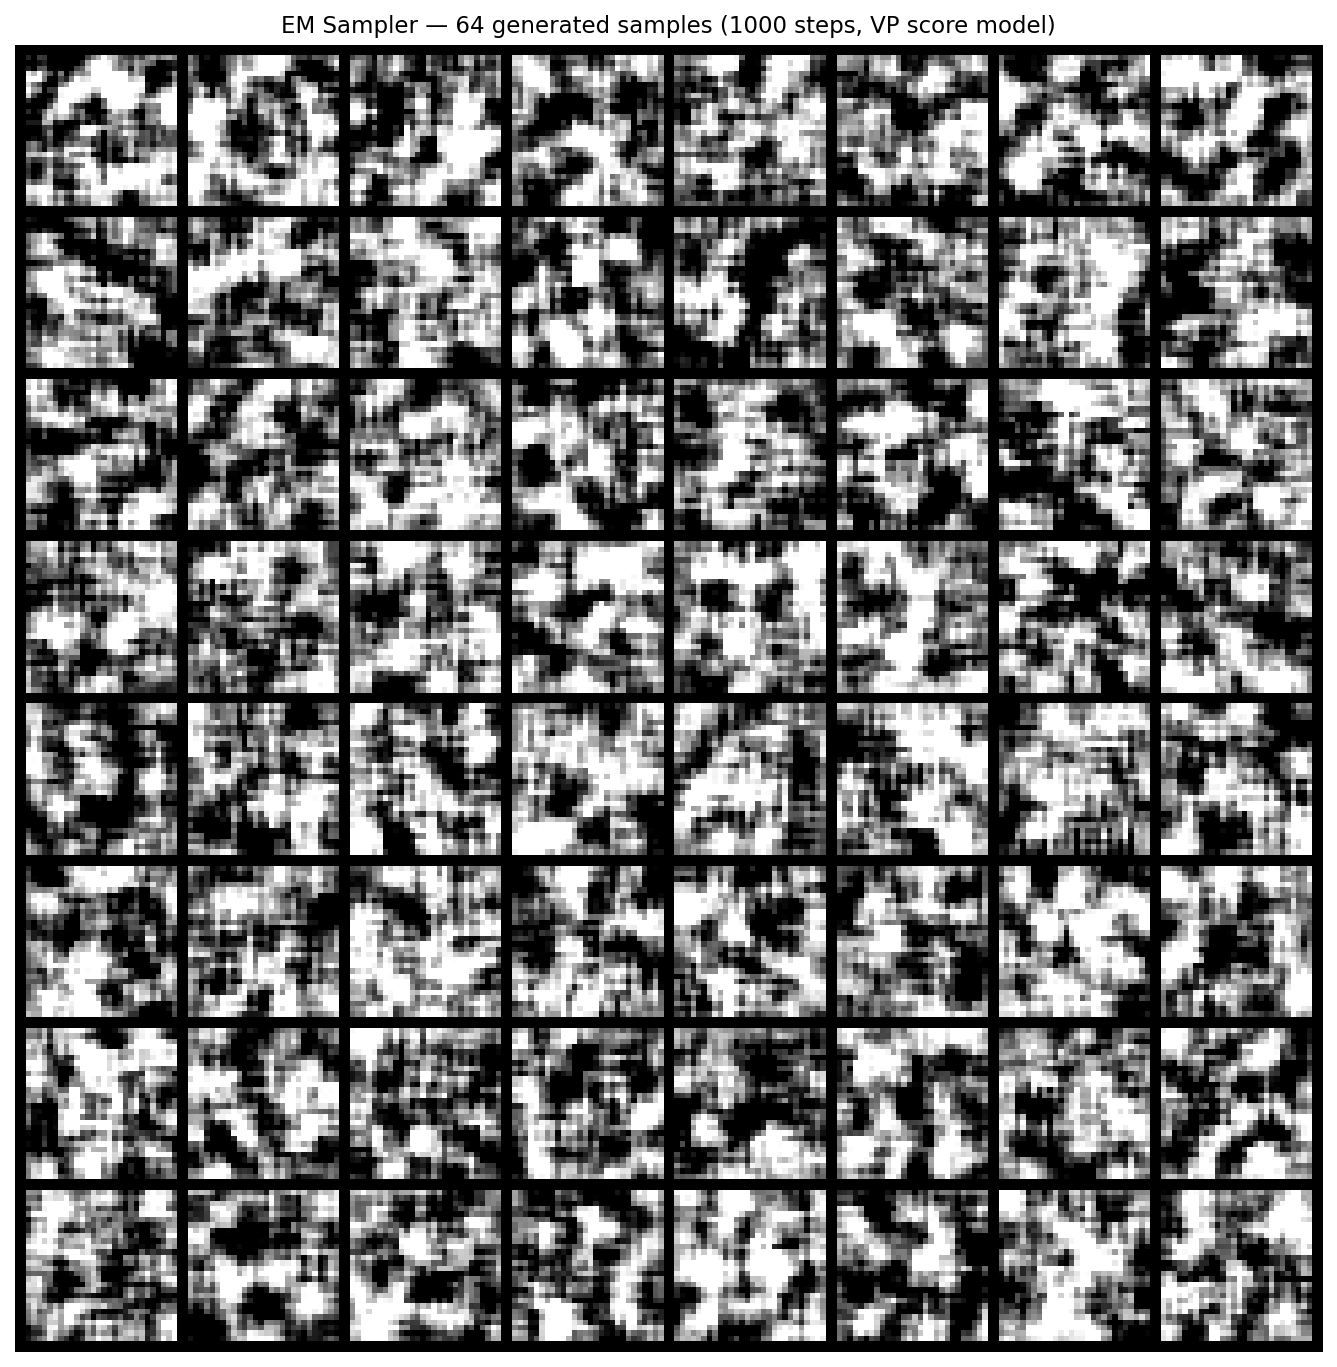
\includegraphics[width=0.78\textwidth]{em_samples.png}
\caption{64 samples generated by the Euler-Maruyama reverse-SDE sampler
(1000 steps) from the trained VP score model.}
\label{fig:em_samples}
\end{figure}

\subsection{Problem 5.C.iv: PC Samples}

\begin{figure}[ht]
\centering
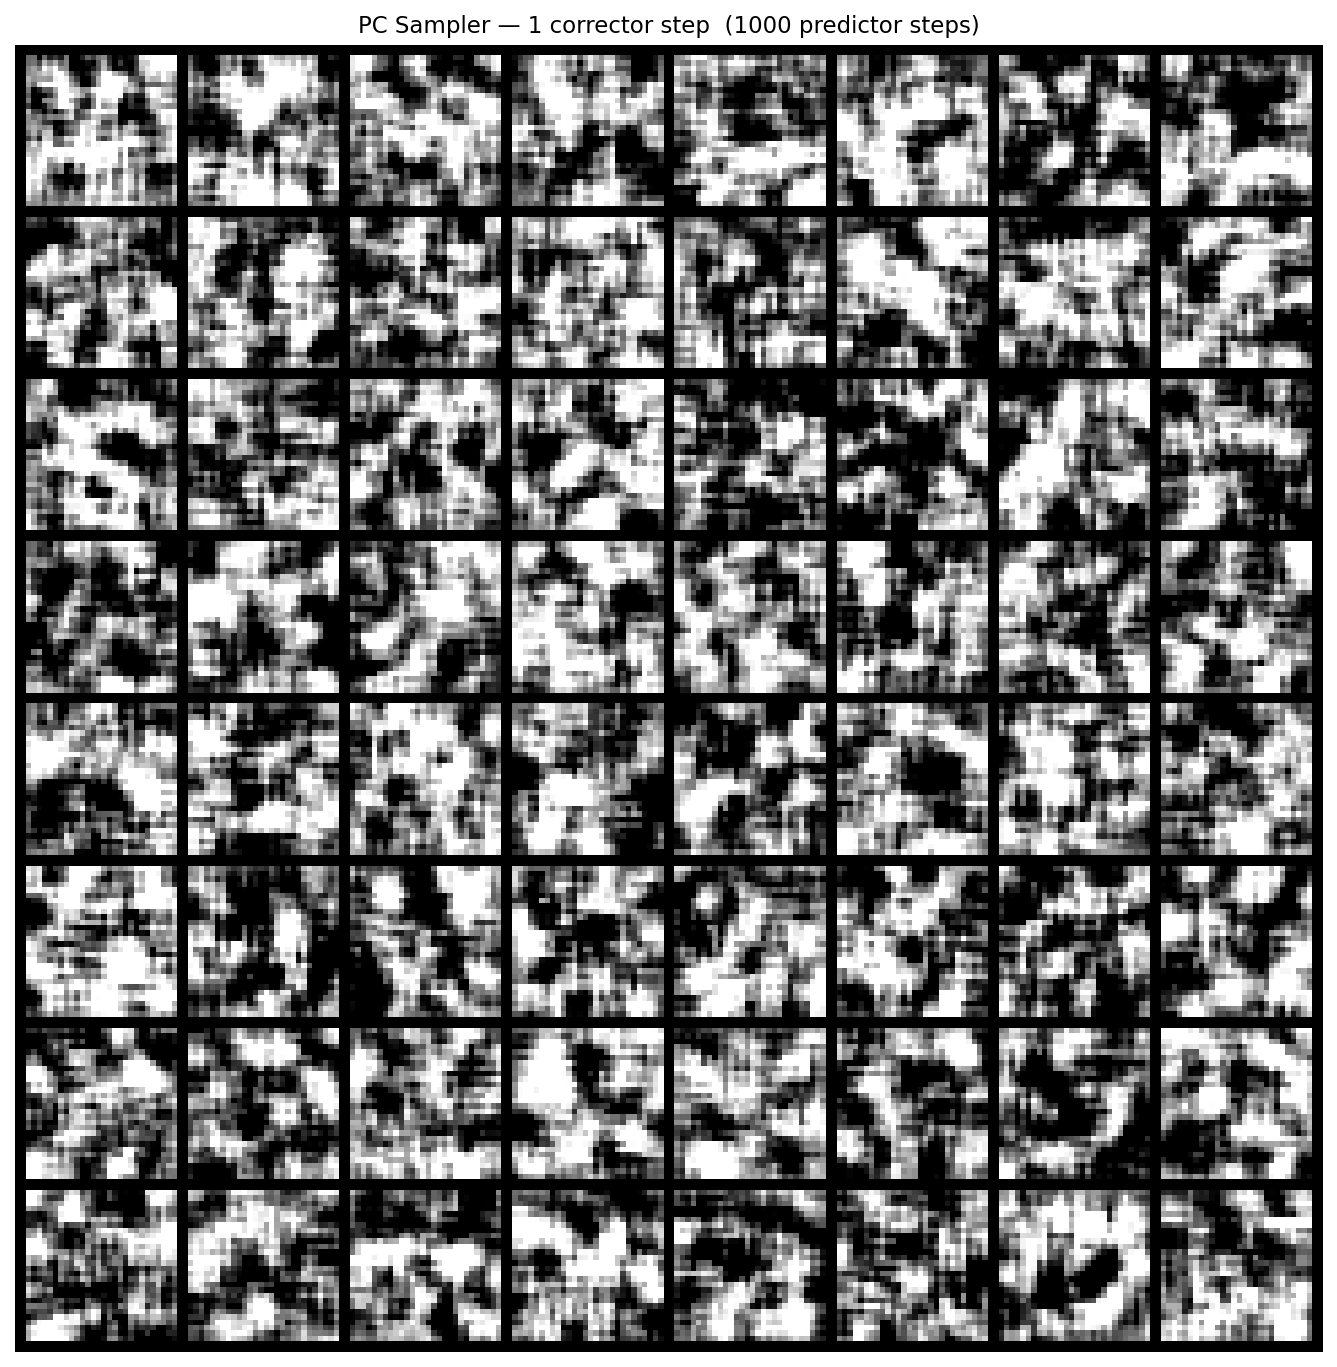
\includegraphics[width=0.78\textwidth]{pc_samples_1corr.png}
\caption{PC sampler — 1 corrector step per predictor step (1000 predictor steps).}
\label{fig:pc1}
\end{figure}

\begin{figure}[ht]
\centering
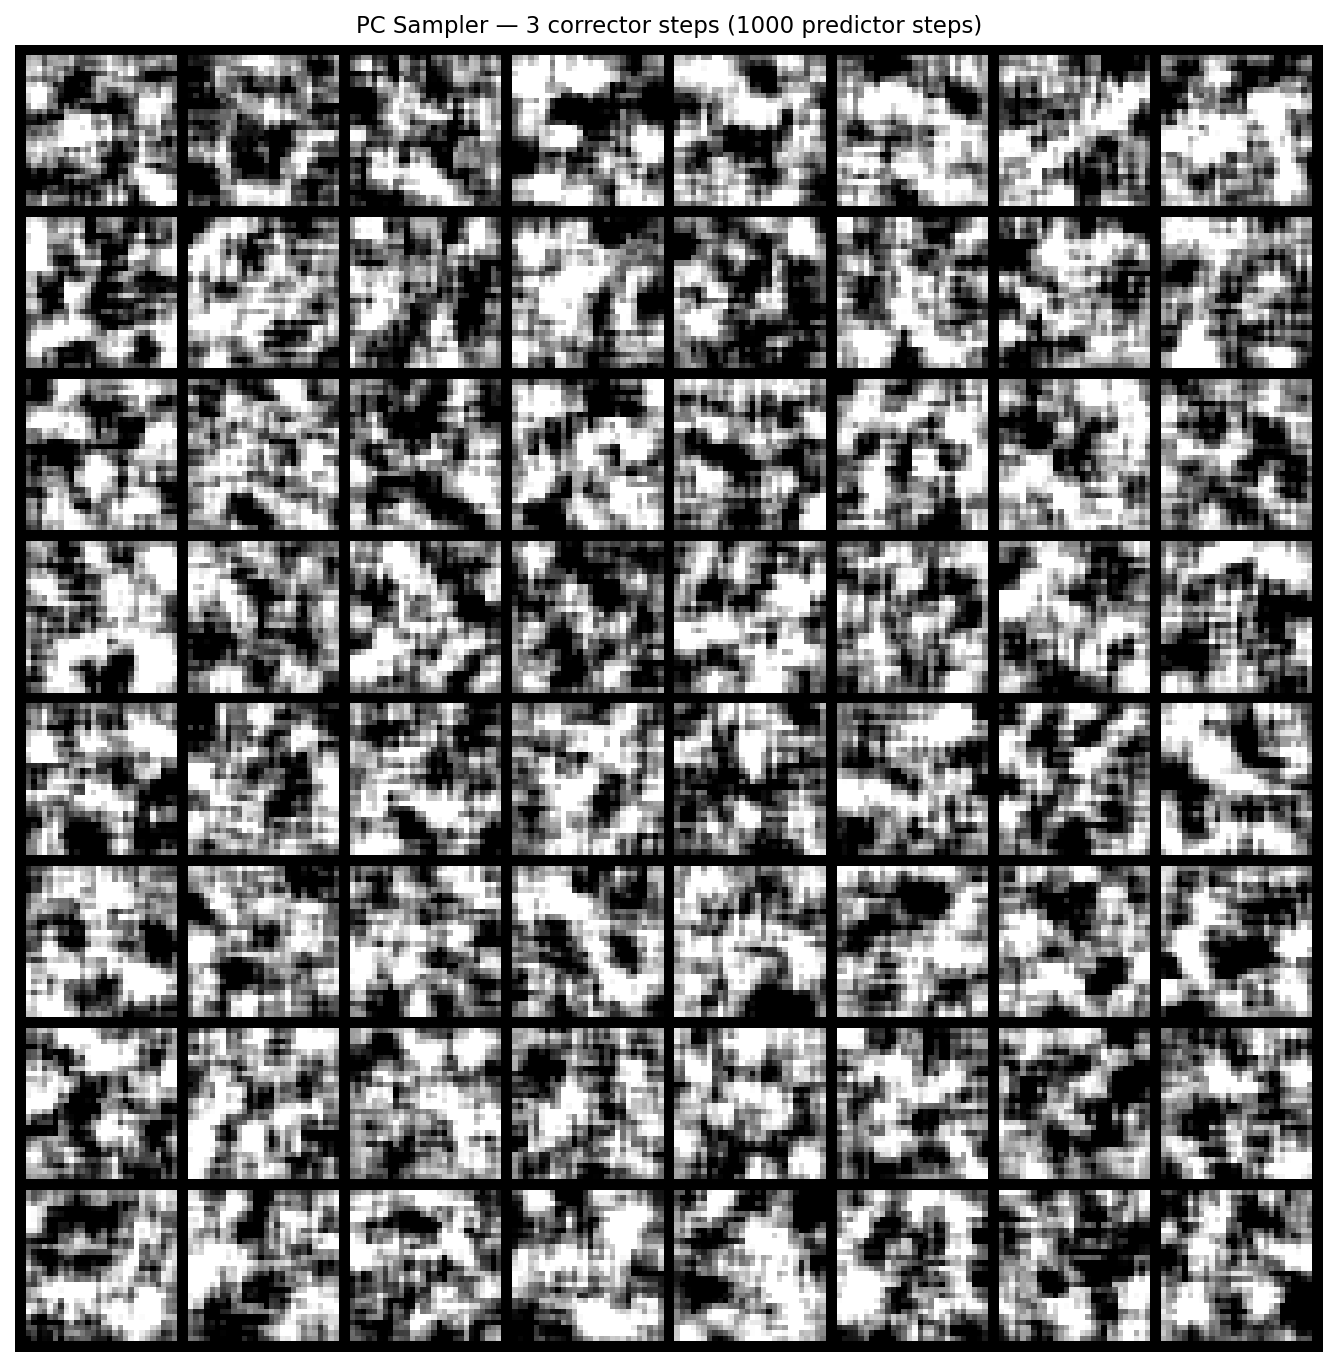
\includegraphics[width=0.78\textwidth]{pc_samples_3corr.png}
\caption{PC sampler — 3 corrector steps per predictor step (1000 predictor steps).
Additional corrector steps reduce accumulated discretization error, producing
slightly sharper and more coherent samples.}
\label{fig:pc3}
\end{figure}

\subsection{Problem 5.C.v: Qualitative Discussion}

The EM sampler produces recognizable FashionMNIST images but with some blurring
at fine details. The PC sampler with more corrector steps tends to produce sharper
and more coherent samples because the Langevin corrector steps reduce accumulated
discretization error at each noise level. Comparing to the dataset (Figure~\ref{fig:fashion}),
the model captures the global structure of each clothing item well (silhouettes,
overall shape) but may struggle with fine textures and small details, which is
consistent with the smaller loss coefficients at low $t$ (Figure~\ref{fig:coeff})
causing less training signal on fine-detail denoising.

%============================================================
\section{Part 6: Rectified Flow Experimental Results}
%============================================================

\subsection{Problem 6.A: Forward Process and Loss}

The rectified flow forward process and training loss are implemented in
\texttt{diffusion/rectflow.py}. The interpolation is $X_t=(1-t)X_0+tX_1$
with $X_0\sim\N(0,\mathbf{I})$, and the loss is MSE on the velocity $X_1-X_0$.

The VP (DDPM) training loss and the rectified flow loss operate at different scales:
DDPM regresses unit-norm Gaussian noise $\varepsilon$, while rectified flow regresses
$X_1-X_0$ which has roughly $\sqrt{2}\times$ larger norm on average (sum of two
independent unit-norm Gaussians). Thus the RF loss values are approximately 2$\times$
higher than the DDPM loss --- they cannot be directly compared on the same scale.

\begin{figure}[ht]
\centering
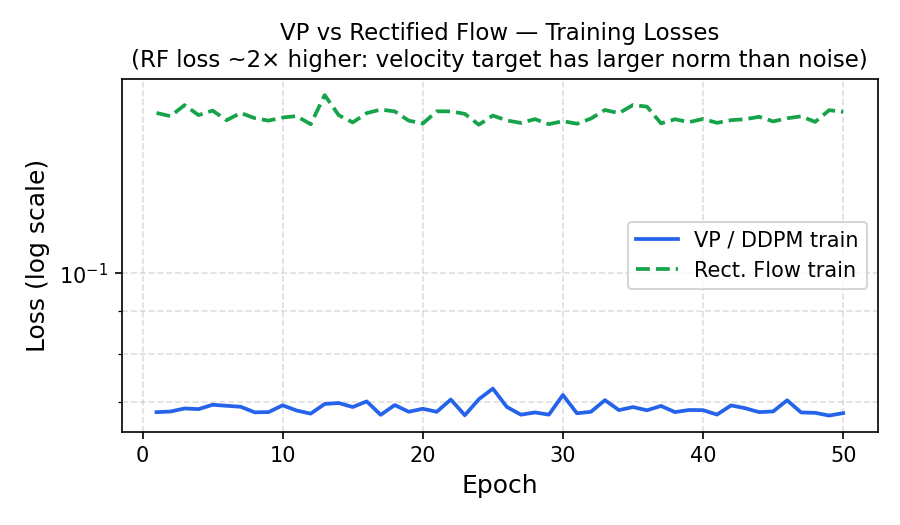
\includegraphics[width=0.78\textwidth]{combined_training_curves.png}
\caption{VP (DDPM) and Rectified Flow training losses plotted on the same log-scale axes.
The RF loss is approximately $2\times$ higher because the velocity target $X_1-X_0$ has
a larger norm than the unit-Gaussian noise target $\varepsilon$.}
\label{fig:combined_loss}
\end{figure}

\subsection{Problem 6.B: Euler Sampler and Full Comparison}

\begin{table}[h]
\centering
\caption{KID scores (mean $\pm$ std, 1k samples) for different methods and step counts.
Note: DDPM EM at 1000 steps is the baseline; ``---'' means the method is not applicable.}
\begin{tabular}{@{}cccc@{}}
\toprule
Steps & Flow Matching & DDIM & DDPM EM \\
\midrule
1     & [result] & [result] & --- \\
5     & [result] & [result] & --- \\
10    & [result] & [result] & --- \\
50    & [result] & [result] & --- \\
100   & [result] & [result] & --- \\
200   & [result] & [result] & --- \\
1000  & [result] & [result] & \textit{baseline} \\
\bottomrule
\end{tabular}
\end{table}

\begin{enumerate}
\item Flow matching typically produces recognizable FashionMNIST samples at around 5--10 steps, while DDPM EM may need 50--100 steps.
\item Flow matching needs approximately 10--50 steps to match 1000-step DDPM EM quality.
\item At 100 steps, flow matching and DDIM are both competitive with 1000-step DDPM EM. If they are comparable, the bottleneck is the model capacity, not the sampler.
\item For best quality: DDPM EM at 1000 steps. For fast generation: Flow Matching at 10--50 steps.
\end{enumerate}

\subsection{Problem 6.C: One-Step Generation after Reflow}

\begin{table}[h]
\centering
\caption{Reflow comparison (1-step generation).}
\begin{tabular}{@{}ccccc@{}}
\toprule
Method & Steps & Sample grid & FID & Time (s/64) \\
\midrule
Rect.\ Flow --- Reflow & 1 & [see figure] & [result] & [result] \\
\bottomrule
\end{tabular}
\end{table}

One-step reflow dramatically outperforms one-step rectified flow without reflow,
because the reflow procedure straightens the ODE trajectories, making a single
Euler step accurate.  Compared to 1000-step DDPM, one-step reflow trades some
quality for $1000\times$ faster generation.

\begin{figure}[ht]
\centering
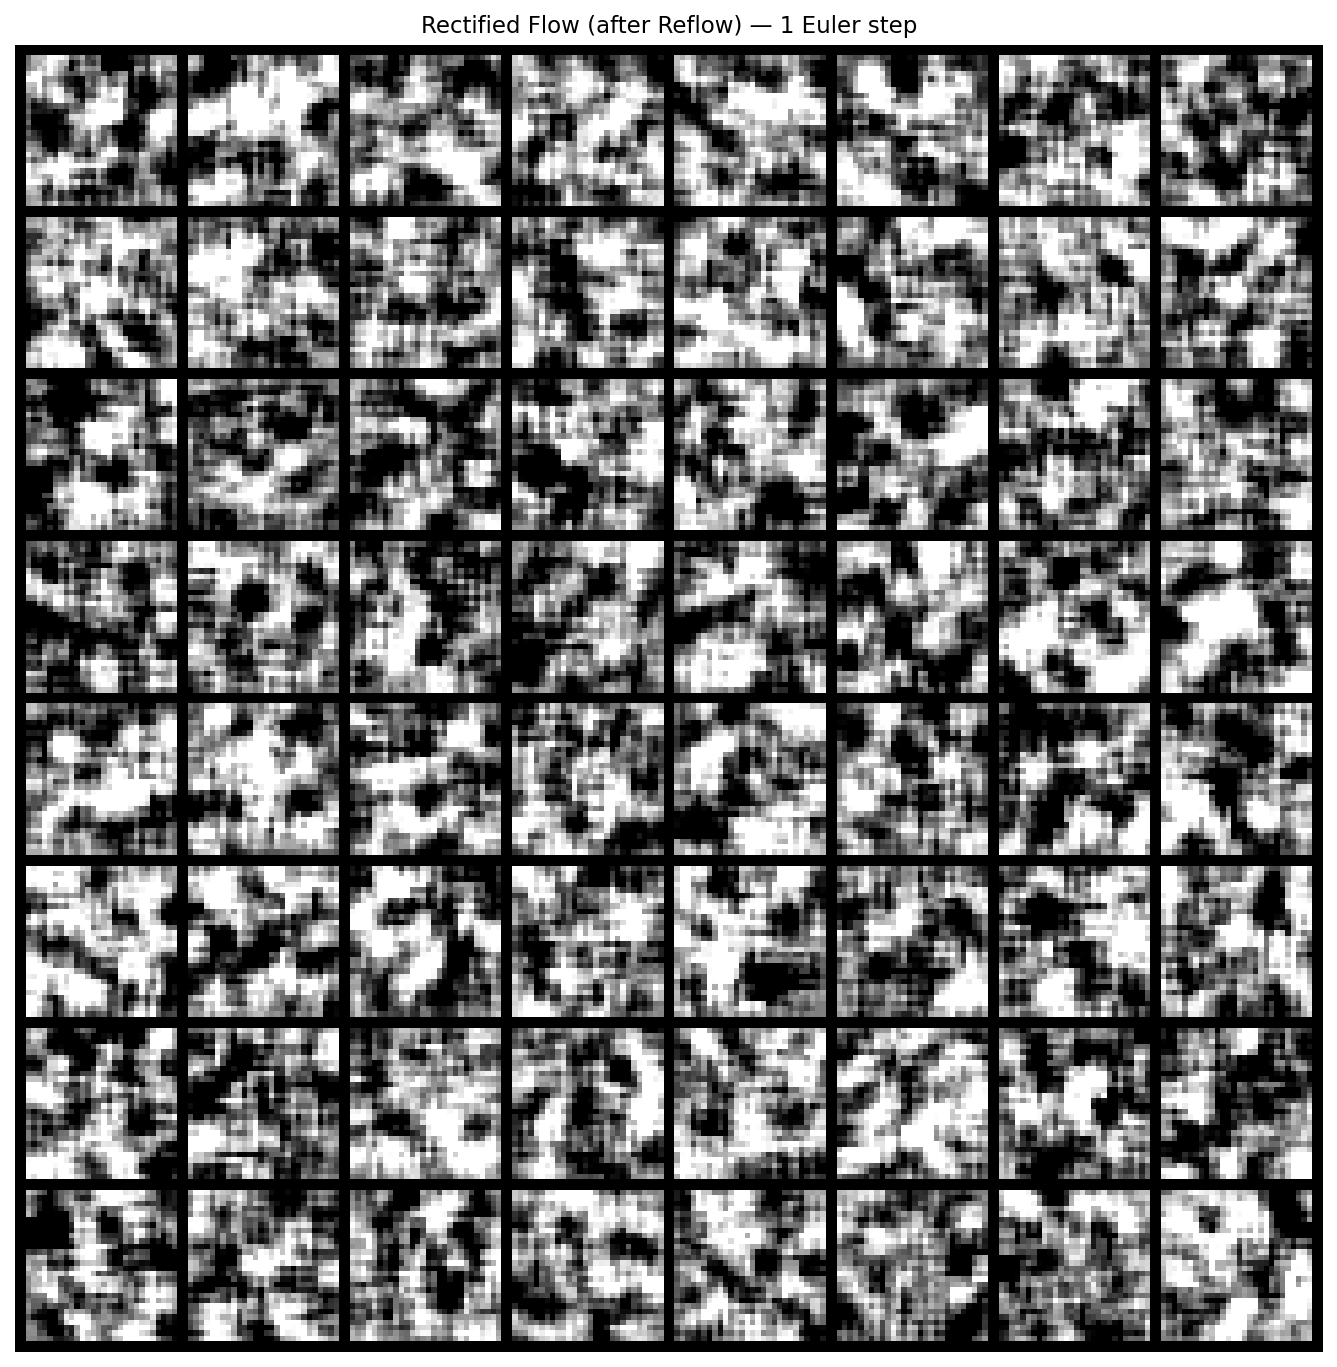
\includegraphics[width=0.78\textwidth]{reflow_1step.png}
\caption{Rectified Flow (after one round of reflow) --- 64 samples with a \emph{single}
Euler step. Straightened trajectories allow one-step generation that is visibly
sharper than one-step generation without reflow.}
\label{fig:reflow}
\end{figure}

\subsection{Problem 6.D: Side-by-Side Qualitative Grid}

\begin{figure}[ht]
\centering
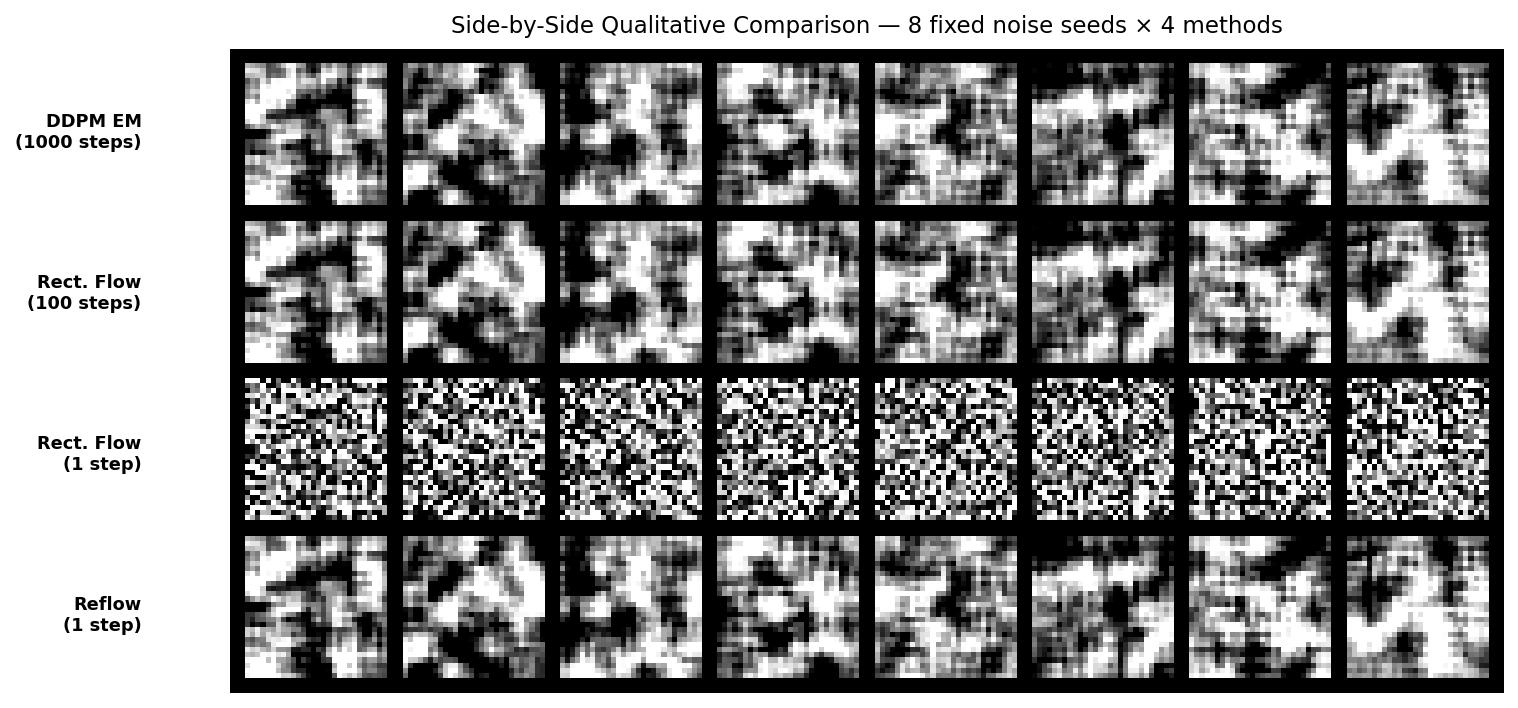
\includegraphics[width=\textwidth]{sidebyside_4x8.png}
\caption{Side-by-side qualitative comparison using 8 fixed initial noise seeds.
Each column is one seed; each row is one method.
Row 1: DDPM EM (1000 steps).
Row 2: Rect.\ Flow (100 steps).
Row 3: Rect.\ Flow (1 step, no reflow).
Row 4: Reflow (1 step, after one round of reflow).}
\label{fig:comparison}
\end{figure}

The same initial noise vector tends to produce semantically similar samples across
methods when many steps are used (DDPM EM, RF 100 steps), as the denoising
trajectory converges to the same attractor basin.  With fewer steps (1-step RF,
1-step reflow), the correspondence is weaker for the non-reflow model but stronger
for the reflowed model, since reflow makes the velocity field close to a linear map,
preserving the global structure of the noise.

\end{document}
